\chapter{Evaluation}
The goal of this paragraph is to assure that the changes we made to AutoWDS basic actually improved its performance.
Due to extent this work is aimed at, it was not feasible to implement all the systems of the related solutions on this field on a common environment
to get a fair assessment for each work. For this the overview papers on this area like \cite{overview_caa} may serve its purpose.
The following subsections will mainly focus on the comparison between AutoWDS basic and the extended version.
\section{Test arrangement}
Since the main goal is to increase overall throughput performance as described in the requirements analysis, our basic evaluation approach is
to find by how much we were able to increase this metric. Therefore we ran both systems under equal circumstances with various settings and multiple runs
and compared its capacities.
  \subsection{Physical Infrastructure}
    For the test arrangement we used the following hardware:
      11 Accesspoints, 1 WLC and 2 Switches among those
      \begin{itemize}
       \item 3 x Lancom L322agn dual Wireless //cite the website or product catalog?
       \item 3 x Lancom L-452agn dual Wireless
       \item 6 x Hirschmann OpenBAT-R
       \item 1 x Lancom WLC-4100
       \item 2 x Lancom GS-2352P
      \end{itemize}
      running on Firmware Version <<insert version here>>. We deployed them at a typical office environment as depicted in the figure.
      Only omnidirectional antennas for the accesspoints were used for this setup. As we had to connect each of the accesspoints also
      per cable to the monitoring station and power grid in order to route traffic through them and the network they're spanning,
      we could not set them further appart.
      Increasing the distance between the single APs would have lead to a sparser network topology and so the hidden station problem would have occured
      more often. Thus the actual interference would have gone up, since with a lower Signal to Noise ratio the APs would not be able to recognize each others 
      transmissions as those and categorize it as interference instead of applying CSMA/CD, leading to more corrupt packets.
      We were able to simulate this problem with a reduced transmit-power,
      but even on the lowest setting most of the accesspoints were able to receive each others beacons. With this limitation kept in mind we expect
      the gap between the two scenarios in the following results to be even greater.
      Since this test was conducted at a research facility for wireless LAN devices, especially the 2.4Ghz band was quite heavily utilized as you will notice
      in the performance charts.
    \begin{figure}[t]
      \centering
      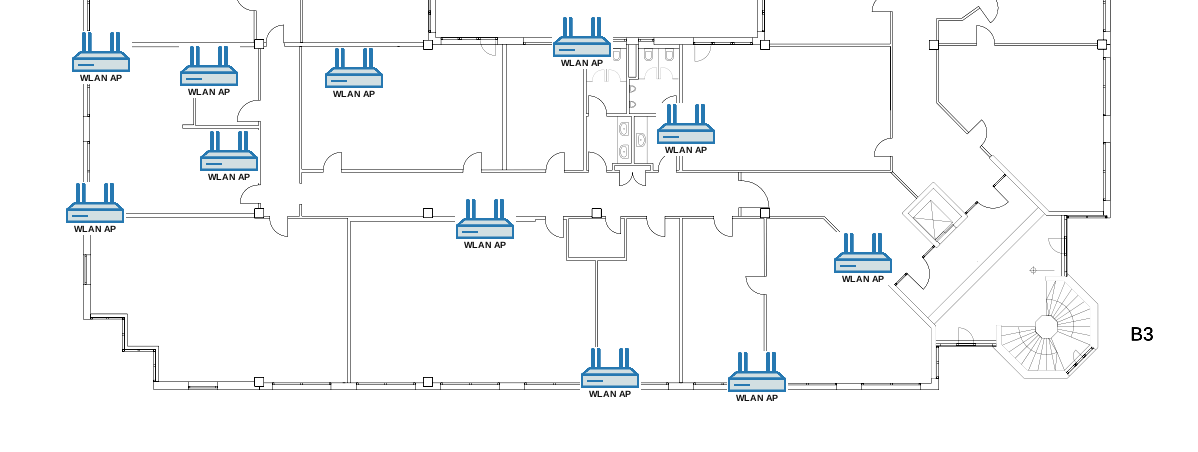
\includegraphics[width=1\columnwidth]{figures/Lancom-flur-withaps}
      \caption{Physical arrangement of accesspoints in an area of rougly 15m x 40m}
      \label{fig:2ndfloor}
    \end{figure}
  \subsection{Network Infrastructure}
    \begin{figure}[h]
      \centerline{
	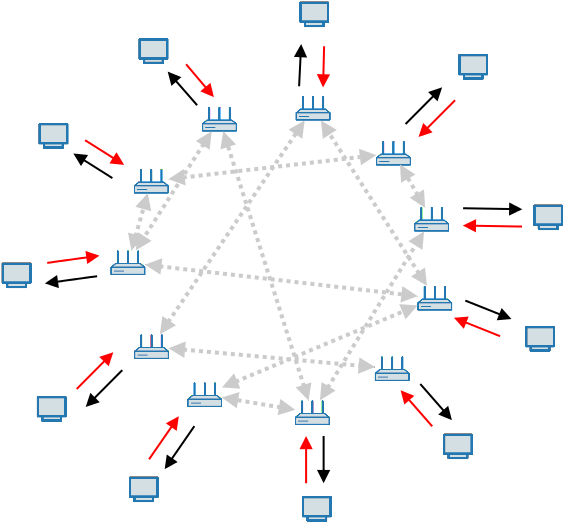
\includegraphics[width=0.3\textwidth]{figures/testsetup_logic}%
	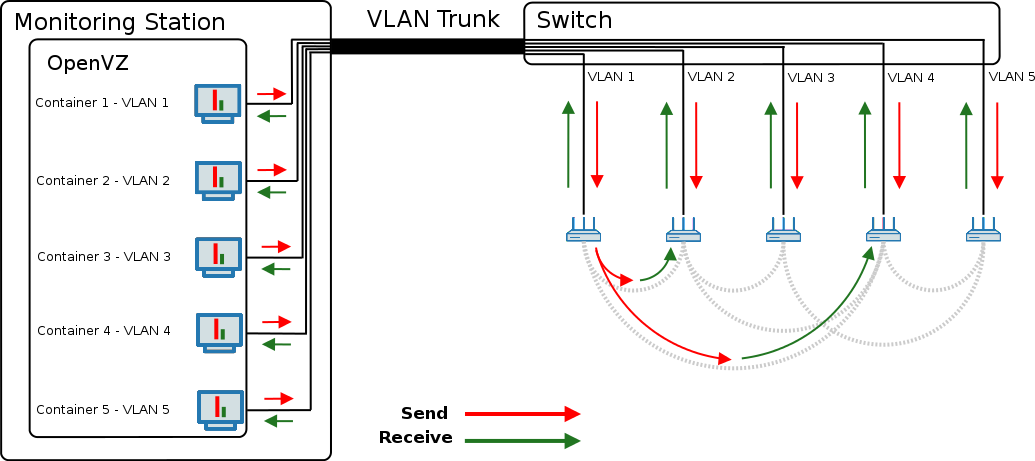
\includegraphics[width=0.7\textwidth]{figures/testsetup_openvz}%
	\caption{Example for the logical arrangement of accesspoints with systems attached by cable, which generate broadcast traffic that is routed through the 
	wireless network spanned by the accesspoints. And on the right side implementation of the test arrangement with available hardware.}
      } % TODO: Bilder besser anordnen/anpassen
      \label{fig:testsetup_logic}
    \end{figure}
    To 
    OpenVZ \newline
    VLAN \newline
    IPerf \newline
\section{Metrics}
  \subsection{Durations}
    \begin{description}
     \item[How long were the tests run?]
      10 Minutes
     \item[Measurement Intervalls]
      7 Seconds
    \end{description}
  \subsection{Channelusage}
    Which Channels were used and in what combinations? \newline
    Image of AutoWDSstatus Topology: (How to place the nodes? What to show?)
      1 \newline
      36 \newline
      1,6,11 \newline
      36,40,44 \newline
      1,6,11,36,40,44 \newline
  \subsection{Characteristics}
    \begin{description}
     \item [When did the tests take place?]
      Mainly Sundays / Holidays in the evening \newline
     \item[Transmission powers used for the tests]
      Antenna gain 3 dB \newline
      Antenna gain 20 dB + Transmitt power reduction \newline
    \end{description}
\section{Results}
  \subsection{Expectations}
    What results would we expect?\newline
  \subsection{Actual Results}
    \begin{description}
     \item [Do the actual results diverge from the expected ones?]
     \item[Assessment of the base scenario]
      Base Scanario (uses only 1 Channel for all connections) pretty much broken by design -> Medium totally overloaded -> does not even scale to 3 APs in close proximity \newline
     \item[By how much is the solution better then before?]
      Despite being actually usable again, Traffic throughput is ~7-10 Times higher
    \end{description}
\section{Reflection on the requirements}
  How far does the solution meet the requirements?\newline
  \subsection{Increased Throughput}
    Definitely, see Diagrams \newline
  \subsection{Reduced Connectivity failures}
    Not tested, since test equippment lacks support for multi-flow/routing support (only bridged connections between APs) \newline
  \subsection{Multiple Radios utilized}
    Surely, with excess radios being usable for client connections \newline
  \subsection{Solution works within the perimeter}
    Absolutely, since we can compute CAA on central entity and works best for static scenarios \newline
  \subsection{Comply with Economic Restrictions}
    Runtime for Small scenarios (about 13 APs with about 500 Possible connections) on a modern system (fill in description of system) small -> <1 Second
    Estimate for bigger scenario missing (How do i correctly estimate that?)
\section{Reflection on related Work}
  Comparison to related Work algorithms\newline
  \subsection{Features of other Systems}
  \subsection{Features of our System}
\section{Discussion}
  \begin{description}
   \item [Checking the coloring and channel assignment after the algo run]
   this might not be the best place for this point, but serves just as a reminder.
   \item [What do the results mean?]
   Obviously it is useful to use mutliple channels for WDS system
   \item[What could'nt we measure?]
   What measurements are still missing:  run testcases for each parameter like formula,...
   Evaluate the redundant paths feature.
   Simulate the system with more accesspoints and various parameteres
  \end{description}